\documentclass[]{article}
\usepackage{lmodern}
\usepackage{amssymb,amsmath}
\usepackage{ifxetex,ifluatex}
\usepackage{fixltx2e} % provides \textsubscript
\ifnum 0\ifxetex 1\fi\ifluatex 1\fi=0 % if pdftex
  \usepackage[T1]{fontenc}
  \usepackage[utf8]{inputenc}
\else % if luatex or xelatex
  \ifxetex
    \usepackage{mathspec}
  \else
    \usepackage{fontspec}
  \fi
  \defaultfontfeatures{Ligatures=TeX,Scale=MatchLowercase}
\fi
% use upquote if available, for straight quotes in verbatim environments
\IfFileExists{upquote.sty}{\usepackage{upquote}}{}
% use microtype if available
\IfFileExists{microtype.sty}{%
\usepackage{microtype}
\UseMicrotypeSet[protrusion]{basicmath} % disable protrusion for tt fonts
}{}
\usepackage[margin=1in]{geometry}
\usepackage{hyperref}
\hypersetup{unicode=true,
            pdftitle={Regression - Final project},
            pdfauthor={Victoire de Termont and Sarah Jallot},
            pdfborder={0 0 0},
            breaklinks=true}
\urlstyle{same}  % don't use monospace font for urls
\usepackage{graphicx,grffile}
\makeatletter
\def\maxwidth{\ifdim\Gin@nat@width>\linewidth\linewidth\else\Gin@nat@width\fi}
\def\maxheight{\ifdim\Gin@nat@height>\textheight\textheight\else\Gin@nat@height\fi}
\makeatother
% Scale images if necessary, so that they will not overflow the page
% margins by default, and it is still possible to overwrite the defaults
% using explicit options in \includegraphics[width, height, ...]{}
\setkeys{Gin}{width=\maxwidth,height=\maxheight,keepaspectratio}
\IfFileExists{parskip.sty}{%
\usepackage{parskip}
}{% else
\setlength{\parindent}{0pt}
\setlength{\parskip}{6pt plus 2pt minus 1pt}
}
\setlength{\emergencystretch}{3em}  % prevent overfull lines
\providecommand{\tightlist}{%
  \setlength{\itemsep}{0pt}\setlength{\parskip}{0pt}}
\setcounter{secnumdepth}{0}
% Redefines (sub)paragraphs to behave more like sections
\ifx\paragraph\undefined\else
\let\oldparagraph\paragraph
\renewcommand{\paragraph}[1]{\oldparagraph{#1}\mbox{}}
\fi
\ifx\subparagraph\undefined\else
\let\oldsubparagraph\subparagraph
\renewcommand{\subparagraph}[1]{\oldsubparagraph{#1}\mbox{}}
\fi

%%% Use protect on footnotes to avoid problems with footnotes in titles
\let\rmarkdownfootnote\footnote%
\def\footnote{\protect\rmarkdownfootnote}

%%% Change title format to be more compact
\usepackage{titling}

% Create subtitle command for use in maketitle
\providecommand{\subtitle}[1]{
  \posttitle{
    \begin{center}\large#1\end{center}
    }
}

\setlength{\droptitle}{-2em}

  \title{Regression - Final project}
    \pretitle{\vspace{\droptitle}\centering\huge}
  \posttitle{\par}
    \author{Victoire de Termont and Sarah Jallot}
    \preauthor{\centering\large\emph}
  \postauthor{\par}
      \predate{\centering\large\emph}
  \postdate{\par}
    \date{12/3/2019}


\begin{document}
\maketitle

Our objective is to predict the prices of residential homes in Ames,
Iowa accurately. Our key metric will be the RMSE on test data.\\
The training data consists of 66 categorical and quantitative variables
extensively describing 1,095 residential homes in Ames, Iowa, and the
houses' corresponding price in dollars. Discriminating between relevant
and non relevant regressors to foster sparsity in our model is paramount
for an efficient and robust model.

We first investigate numerical and factor variables sequentially.
log(SalePrice) is close to a Gaussian distribution, with a few extreme
outliers. A PCA on numerical variables shows that 19/23 numerical
variables account for 99\% of the sample variance. We distinguish three
types of factors: factors with an overrepresented level, some with high
cardinality, and others with standard level repartition. We then perform
elementary factor pruning and intra-factor modality regrouping before
using ANOVA to remove factors manually. We do not touch numerical
variables but instead rely on our model to make a selection.\\
We fit two linear models using stepwise selection procedure with the AIC
criterion to foster sparsity. In the first model, we predict
log(SalePrice), before removing outliers after testing them. In the
second model, we winsorise log(SalePrice) as we noticed that extreme
outliers made our model less robust. In both cases we retain the
backward selection model. Model 1 predicts the test data much more
accurately than model 2 (24 000\$ vs 33 000\$), but model 2 validates
the regression assumptions more clearly. We retain model 1: it
generalises better, and meets the postulates. Our predictions are much
better under the 300K threshold for SalePrice. Had we had enough
datapoints, we could have fitted two models: one for values underneath
and above that threshold.

\textbf{I. Introduction - Data description}\\
We first contextualise the pre-processed data.

The data we are handling is heterogeneous, although it is presented in a
structured manner. We are dealing both with categorical and quantitative
variables, which we will consider separately.

We observe in the data summary that a full model would include 66
features and an intercept, and 1,095 observations. The list of features
is extensive: not all regressors will be useful to predict house price.
We expect the variable MSZoning to have much more impact on the price
that the variable Heating, as the heating system is something that can
be changed, whereas the location is permanent. Note that quantitative
variables differ in scale and range: prices start from
\textasciitilde{}35,000 dollars, and can attain 755,000. Before
pre-processing, surfaces took higher values than bedrooms above ground
which ranged from 1 to 8. Scaling the data allows to reflect the true
impact of each regressor on the output.

R casts some factors as integers: mainly areas and ratings. We decide
not to consider years as factors for our predictions to generalise to
unencountered years. We recast OverallQual, OverallCond, MoSold,
MSSubClass and Fireplaces as factors. We keep other quality-driven
variables as numerics to keep model robustness. All quantitative
features are integers and price, the output, is the only numeric. R
automatically encodes factors: we choose to keep the by default levels,
which are alphabetically ordered.

We check there are no missing values in the pre-processed data before
launching into the analysis: there are 0 missing values in our
dataframe.

\textbf{II. Exploratory data analysis - Initial modeling} 1. Numerical
analysis.\\
We find that we should predict log(SalePrice) to liken it to a gaussian.
We then analyse the feature correlation matrix and perform a PCA: 19/23
numerical variables account for 99\% of the variance. We left it out for
concision but it is graphically available in the code. We count on
stepwise selection to eliminate superfluous numerical regressors.

We first observe the output, SalePrice.

\begin{center}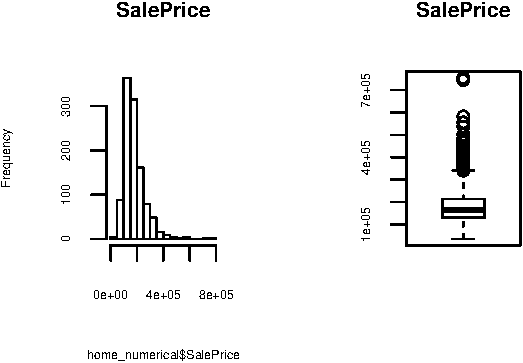
\includegraphics{r_file_v5_files/figure-latex/unnamed-chunk-7-1} \end{center}

SalePrice skewness is very high at 1.92 : Saleprice mean is
\textasciitilde{}181,196 whereas the median is much lower at
\textasciitilde{}164,500. We may have trouble predicting RHS extremes.
To smoothen the output and we will consider the log(SalePrice). If this
isn't enough, we could go a step further by either trimming or modifying
outlier values to improve our generalisation error.

\begin{center}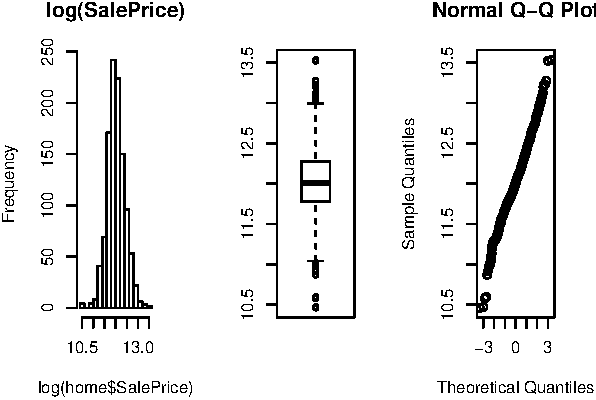
\includegraphics{r_file_v5_files/figure-latex/unnamed-chunk-9-1} \end{center}

log(SalePrice) is pretty close to a normal distribution, except for
extreme values.

\begin{center}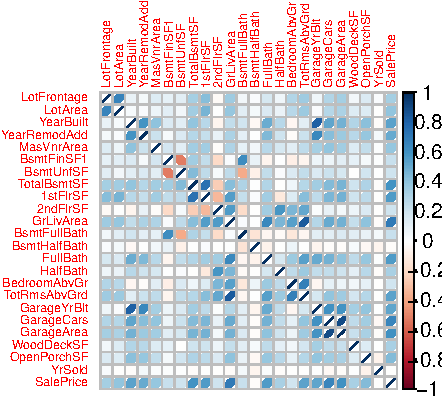
\includegraphics{r_file_v5_files/figure-latex/unnamed-chunk-10-1} \end{center}

The numerical features that are the most correlated with SalePrice are:
GrLivArea, GarageArea and GarageCars, 1st \& 2ndFlrSF, YearBuilt
GarageYrBuilt \& YearRemodAdd. Areas and surfaces are all related to
square feet, which we know is a key driver in house sales. The
construction or modernisation works are an indicator of overall quality
of the housing and the investments that went into it, so it makes sense
for them to be correlated to SalePrice. On the contrary, YrSold and
BsmtHalfBath are poorly correlated to SalePrice. YrSold is correlated to
none of the other features, so it is an irrelevant regressor: the
decision to sell a house doesn't have much to do with what drives its
price or the price one can sell it at. The correlation matrix does not
take into account feature interactions, so we will leave numerical
feature selection to our stepwise model procedures.

Our intuition is that three feature types mainly drive SalePrices:
area/surface, location and quality. Let's describe 1stFlrSF as it is the
closest feature to square feet with 2ndFloorSF.

\begin{center}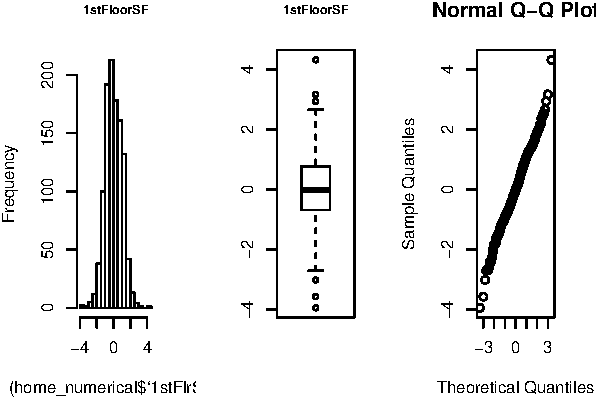
\includegraphics{r_file_v5_files/figure-latex/unnamed-chunk-11-1} \end{center}

From these three graphs, we can assume a Gaussian distribution on
1stFloorSF.\\
Because PCA works best with (scaled) numerical data, we perform it on
the numerical features of our preprocessed data. 19/23 numerical
variables account for \textasciitilde{}99\% of the variance.

\begin{enumerate}
\def\labelenumi{\arabic{enumi}.}
\setcounter{enumi}{2}
\tightlist
\item
  Factor analysis.\\
  We first investigate level fragmentation within the factors. We
  discover three types of factors, as per examples below.
\end{enumerate}

\begin{center}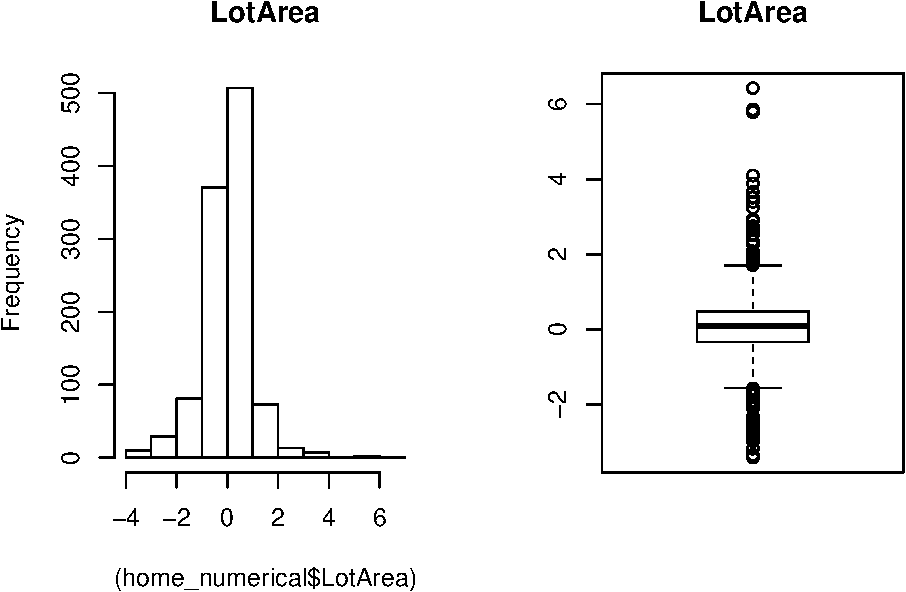
\includegraphics{r_file_v5_files/figure-latex/unnamed-chunk-13-1} \end{center}

\begin{enumerate}
\def\labelenumi{\roman{enumi})}
\tightlist
\item
  Clear underrepresentation of some levels: in Street and Utilities,
  which are binary, this is conspicuous. From this we infer that these
  factors will not be useful in predicting house price in general:
  nearly all houses will be in the same category along these factors
  (and for those who are not, data is too sparse to generalise well).
  Note that this is also the case for RoofMatl, Heating, BsmtFinType2,
  Electrical, GarageCond, GarageQual.\\
\item
  High cardinality in the number of levels: this is especially the case
  for neighbourhood, which has 25 levels. We regroup some of these
  levels together to improve our predictions.Note that this is also the
  case for Exterior1st, Exterior2nd, BsmtExposure.
\item
  Classic factor repartition with reasonable representation of each
  modality, as is the case for Housestyle for instance. Note that this
  is also the case for HeatingQC, GarageFinish, BsmtFinType1.\\
  Intuitively, we said that both location and overall quality will
  impact SalePrice significantly. Let us check this with anova and
  ancova tests.
\end{enumerate}

\begin{center}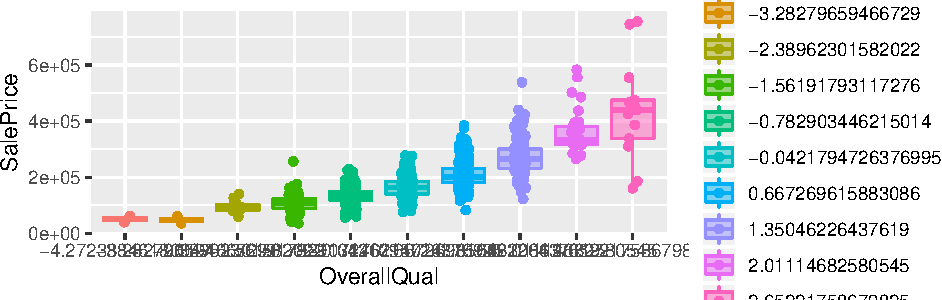
\includegraphics{r_file_v5_files/figure-latex/unnamed-chunk-15-1} \end{center}

Graphically, we see that overall quality ratings have significant impact
over the median SalePrice.

We run two ANOVA tests (available in the code) to confirm that area and
overall quality both individually have a strong effect on SalePrice: we
get a p-value of order e-16.

Our ANCOVA shows that MSZoning, OverallQual and their interaction are
highly significant towards explaining SalePrice. So we will keep these
factors.

\textbf{III. Modeling and diagnostics}\\
We implement stepwise selection with an AIC criterion for sparsity. We
predict SalePrice's logarithm to improve our target smoothness and
estimated residuals homoscedasticity. In our first model, we notice that
our 8 outliers are located towards the bottom values of SalePrice. They
prevent us from validating our postulates, mainly homoscedasticity and
gaussianity. Removing them gives a more robust model, but we thought of
fitting a second model where instead of removing the outliers after
model fit, we use the winsor method to reaffect extreme values and
normalise our data before model fit. Doing this improves model
robustness (the postulates) but also meaningfully increases our MSE on
test data.

We noted earlier that many categorical variables could be considered
uninformative or redundant. - We removed factors with massively
overrepresented categories: Street, Utilities, RoofMatl, Condition2,
Heating, Electrical, Functional, GarageCond.\\
We also made some regroupments within factors to diminish cardinality,
mostly for neighbourhood by creating two new categories: under 20 and 50
sales. - Based on Anova tests, we removed other factors to improve model
robustness: OverallCond, Exterior1st, Exterior2nd. OverallCond in
particular was too specific and weakened our model by creating
observations with leverage one.

\begin{verbatim}
## Analysis of Variance Table
## 
## Response: SalePrice
##                           Df     Sum Sq    Mean Sq  F value    Pr(>F)    
## OverallQual                9 4.5195e+12 5.0216e+11 251.2801 < 2.2e-16 ***
## OverallCond                8 2.1085e+10 2.6357e+09   1.3189    0.2299    
## OverallQual:OverallCond   32 1.6090e+11 5.0280e+09   2.5160 8.352e-06 ***
## Residuals               1045 2.0884e+12 1.9984e+09                       
## ---
## Signif. codes:  0 '***' 0.001 '**' 0.01 '*' 0.05 '.' 0.1 ' ' 1
\end{verbatim}

\begin{itemize}
\tightlist
\item
  For some features, we were not sure wether or not they had an
  influence, so we tested the model with and without them and removed
  them if they were not improving our score : HeatingQC, SaleCondition,
  BsmtFinType2, RoofStyle, ExterQual.
\end{itemize}

After working on our factors, we start by fitting a full linear model to
predict log(SalePrice).

Running a model with all the variables excluding the ones we just
removed, we obtain an adjusted R-squared of 0.91. Many variables could
be removed from our model while marginally affecting its efficiency to
explain SalePrice. To improve model efficiency, we perform a selection
of variables based on forward, backward and both methods.

We choose the model with the smallest AIC.

\begin{verbatim}
## [1]   148.000 -4420.497
\end{verbatim}

\begin{verbatim}
## [1]   106.000 -4469.426
\end{verbatim}

\begin{verbatim}
## [1]   106.000 -4469.426
\end{verbatim}

The 34-feature model including the intercept extracted by backward and
both is the same. Its AIC is smaller than the one of the forward method.
We arbitrarily select the backward model. Let's verify the postulates.\\
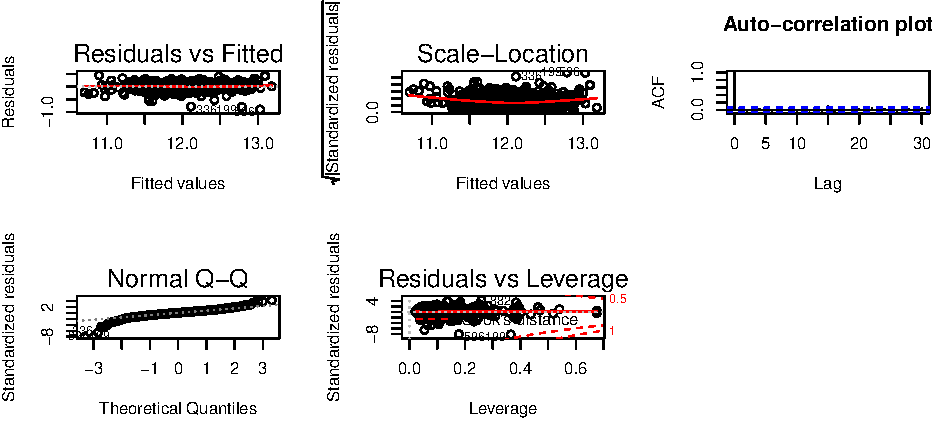
\includegraphics{r_file_v5_files/figure-latex/unnamed-chunk-26-1.pdf} We
validate P1, centered errors, without hesitation. We notice a slight
elliptical behaviour of our residuals in the Scale-Location plot,
potentially problematic for P3 or residual homoscedasticity. Our model
may predict extreme SalePrice values less well than others. However, we
validate the postulate given the plot range of that behaviour (between 1
and 1.5). Observations 336, 199 and 596 have particularly high
standardised residuals. We do not validate P3, the uncorrelation
assumption - one bar exceeds the fitted-line threshold. P4 can be
validated, but again we notice the strange behaviour of tail values,
towards the left-hand-side this time. Points which are not aligned with
the normal distribution quantiles are limited given the number of
observations we have. Note however that observations 199, 336 and 596
appear again: they are far from the theoretical quantiles. None of our
observations has a Cook distance bigger than one. Observation 199 is the
closest to this threshold, meaning it has significant leverage and
residual abnormality.The second closest is observation 596, again. Let's
perform an outlier analysis to see if this helps to validate our
postulates.

\begin{center}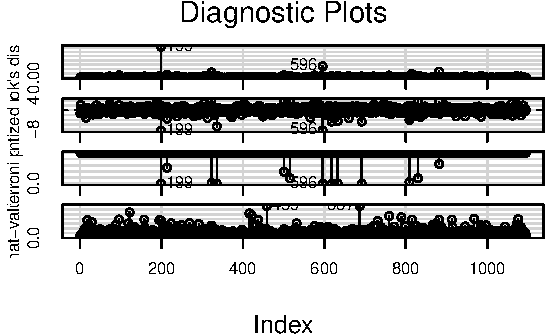
\includegraphics{r_file_v5_files/figure-latex/unnamed-chunk-27-1} \end{center}

Unsurprisingly, observations 199 and 596 are very clear outliers in
nearly all our tests. In the Cook's distance plot, they are close to the
1 threshold albeit under it. Their studentised residuals values are
smaller than -8 (versus a -2 assumption for a 95\% confidence interval),
Bonferroni is of order e-13, the hat values of order e-16. Studentized
residuals plot: 30 points are below -2, and 23 are over 2. Our model
allows for \textasciitilde{}55 outliers within a 95\% confidence
interval and we are within that threshold. Extreme values are
preoccupying: observations 199, 336, 596, 618, 633, 692 and 809 are
smaller than -4. Bonferroni's plot : 6 points have a p-value inferior to
0.5, so they are outliers according to this criterion.\\
Hat plot: observations 459 and 687 have leverage at 0.68, well over 0.5.

An outlier test confirms that 199, 596 and 336 are very clear outliers
and they have significant leverage. So we remove them without question.
The other outliers we get by the outlier test are outliers by far also,
so we remove them.

We now have an adjusted r-squared of 93\% on train data.\\
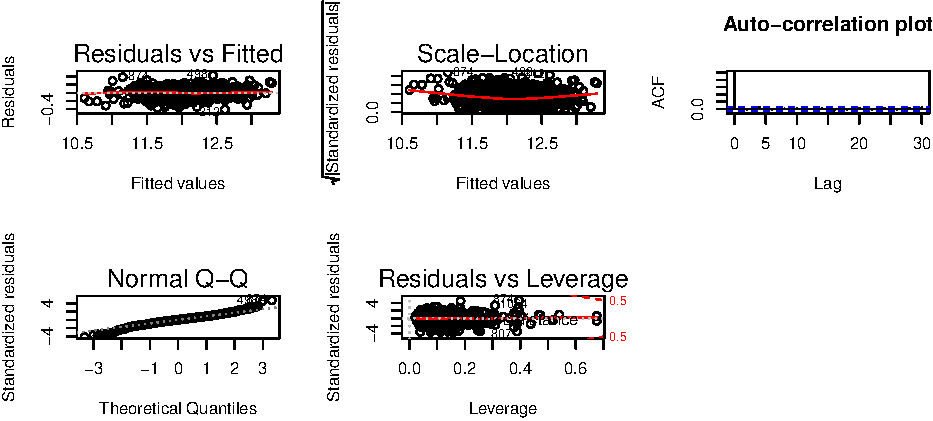
\includegraphics{r_file_v5_files/figure-latex/unnamed-chunk-34-1.pdf}
The postulates are about verified for this model. Residuals are
centered. Scale-location is still slightly elliptic, but we accept it.
We now validate autocorrelation.Gaussianity still poses problem for tail
values. And no observation has significant Cook distance.

We now perform winsorisation on SalePrice and fit a new model.

We have an adjusted r-squared of 91\% on train data.
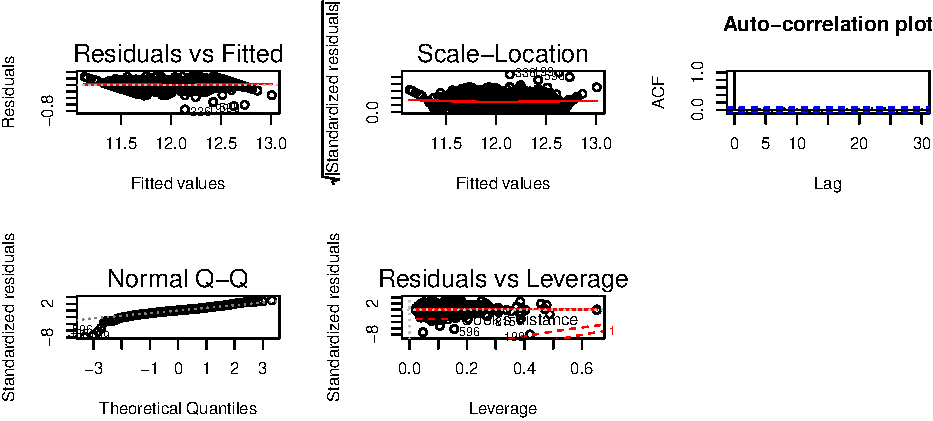
\includegraphics{r_file_v5_files/figure-latex/unnamed-chunk-37-1.pdf}
This time, residuals are perfectly centered. We validate
homoscedasticity and uncorrelation without question. Gaussianity is
still troublesome for tail values. No observation has significant Cook's
distance. Again, observations 336, 199, 596 can be singled out on all
plots.

\begin{center}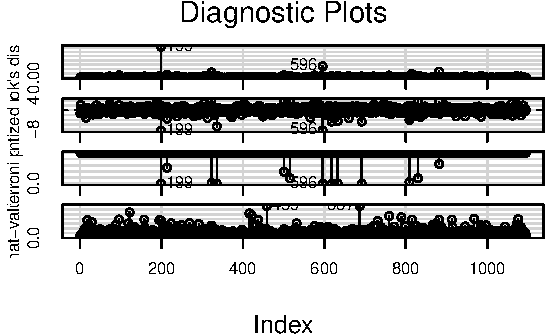
\includegraphics{r_file_v5_files/figure-latex/unnamed-chunk-38-1} \end{center}

We perform the outlier test to confirm our outliers. Without surprise,
199, 336 and 596 are regression outliers. 633 also is. We remove them.

Our winsorised model has a 93\% R-squared on train data once we remove
the outliers.

By a visual analysis we do not display here but available in the code,
we approximately validate our last problematic postulate, Gaussianity.

\textbf{IV. Final models}

RMSE for model 1 is \textasciitilde{}24,5K dollars and RMSE for model 2
is
31.0K\(. Even though our first model is less robust than the second, its test error is much lower. So this is the one we will retain since it still validates our postulates. Let us analyse its coefficients in detail. Model 1 has a 92% adjusted R-squared on train, validation of our postulates and a 24.5k dollar RMSE on test, it is the model that we keep. Its most important features are: Location and area (MSZoning, neighbourhood); Quality and condition (OverallQual,GarageQual, KitchenQual); YearBuilt and YearRemodAdd. As expected, location , quality and condition, and construction/improvement year are our most important features with a high level of significance. Model 2 has a 93% adjusted R-squared on train, validates the postulates, and has a 31.0K\)
RMSE on test. Again we see location with neighbourhood and quality
(OverallQual, GarageQual) as important predictors. In both cases,
testing our model against the intercept we obtain a p-value of order
e-16: we confidently reject that the intercept-reduced model is better
to explain SalePrice than our model.\\
Confidence intervals: as model 1 is mostly impacted by factors, doing
confidence intervals does not help us visualize the proximity among
SalePrice and the most important features. However, doing a 95\%
confidence interval with LotArea, we notice that this variable is not
good at explaning SalePrice by itself, as the price can double for a
same value of LotArea.

\begin{center}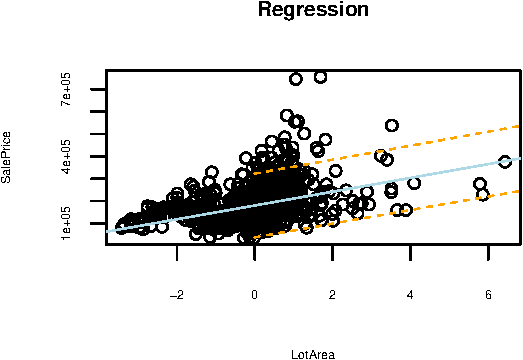
\includegraphics{r_file_v5_files/figure-latex/unnamed-chunk-46-1} \end{center}

\textbf{V. Discussion}\\
Compared to the full linear model run on the-processed dataset, our
postulates are now much better validated with twice as less features (33
instead of 67).\\
Plotting our errors as a function of SalePrice shows that we perform
well under 300K dollars, and badly above with very high residuals for
extreme values, which skews the RMSE towards the top. The graph is
available in the code. Our average residual error is of 18K for
properties under 300K dollars, and 55K for properties above.

A solution would be to fit a model on SalePrices that are above this
threshold, another one on those under, and then average their
predictions to make our final model. As we could infer from the plot,
the skewness of our test residuals is very high at 4.5.

Given that we still use 33 regressors, averaging the predictions of a
lasso, a ridge and an elastic net performed on the features of model 1
could have been another solution to improve predictions and model
robustness. We tried to do so but had struggles plotting our postulates
afterwards, and therefore could not conclude.

\textbf{VI. Bonus}\\
Here is a quick try at implementing the first solution:


\end{document}
